\documentclass{article}
\usepackage[utf8]{inputenc}
\usepackage{graphicx}
\usepackage{multicol}
\usepackage{caption}
\usepackage{subcaption}
\usepackage{wrapfig}
\usepackage{float}
\usepackage{arydshln}
\usepackage{amsmath,amsthm,amssymb,amsfonts}
\usepackage{hyperref}
\usepackage{makecell}
\usepackage{listings}
\usepackage{epsfig}
\usepackage{color}
\usepackage{natbib}
\usepackage[table]{xcolor}
\usepackage[margin=1.1in]{geometry}
\usepackage[affil-it]{authblk}
\newtheorem{theorem}{Theorem}
\newtheorem{lemma}{Lemma}



\def\T{{\mathrm{\scriptscriptstyle T}}}
\def\bmath#1{\mbox{\boldmath$#1$}}

\bibpunct{(}{)}{;}{a}{}{,}
\setlength{\bibsep}{4.0pt}
\renewcommand{\baselinestretch}{1.1}


\title{\textbf{Analysis of Job Influence on Boise House Prices}}

\author{\vspace{11pt}Bridgette Delight}

\affil[1]{Department of Mathematics, Boise State University, Boise, Idaho 83725}
\affil[2]{Department of Computer Science, Boise State University, Boise, Idaho 83725}

\date{\today}


%------------------------------------------------------------------------------%
\begin{document}
%------------------------------------------------------------------------------%

\maketitle

\begin{abstract}

\end{abstract}

\vspace{8pt}
\noindent
KEY WORDS: Key word one; Key word two; Key word three; Key word four.

\section{Introduction}
Over the past eight years, home prices in the Boise metro area have increased very rapidly, outpacing even some of the largest real estate markets in the country. I was interested in seeing what factors might be influencing this rise, and decided to investigate changes in the Boise Metro Area job market to see if changes in employment types could be leading to the rise in prices. This paper will be comparing changes in Tax Assessed Values (TAV) from 2000-2018 with the changes in Employment by sector over the same time period. 

Earlier this year, the Brookings Institution published a study on employment growth across the nation, and used Boise as one of the case studies. Their analysis highlighted some of the areas where Boise's employment opportunities are growing, as well as the ones that are shrinking. I will use this data as a starting point to determine which sectors to analyze in more detail.

https://www.idahostatesman.com/news/business/article230753284.html

https://www.brookings.edu/wp-content/uploads/2019/05/GrowingCitiesthatWorkforAll-FINALforWeb.pdf

\section{The Data}
For the employment numbers, I obtained full data sets from the Bureau of Labor Statistics. This data included a break down by sector, but the sectors didn't directly correspond to the sectors highlighted by the Brookings report. <<Insert how we matched>>

The data for housing prices was obtained from the Ada County Assessor's office. I decided to use the change in Tax Assessed Value (TAV) of properties within Boise, as broken down by the MLS Areas of Boise shown in Figure \ref{fig: mls_map}. TAV was selected over market value because the data set is much more complete, and less subject to bidding fluctuations. There were some outliers that had to be removed, such as lots where new homes were constructed.  

\begin{figure}[H]
    \centering
    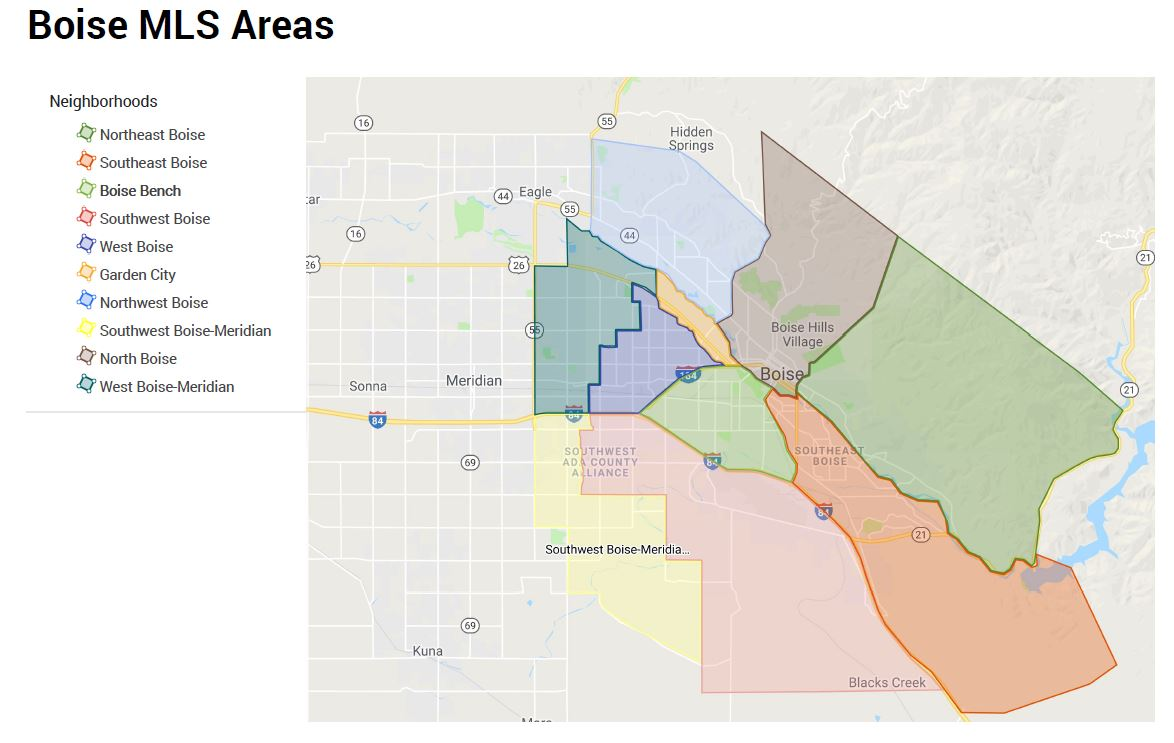
\includegraphics[width= .8\linewidth]{images/MLS_Areas.JPG}
    \caption{MLS Areas of Boise}
    \label{fig: mls_map}
\end{figure}

\begin{table}[H]
    \centering
    \resizebox{.5\textwidth}{!}{
    \begin{tabular}{|l|}
    \Xhline{1 pt}
    \textbf{Job Categories}\\
    \Xhline{1 pt}
    Architecture And Engineering Occupations \\
    \Xhline{1 pt}     
    Arts, Design, Entertainment, Sports, And Media $\dots$\\
    \Xhline{1 pt} 
    Building And Grounds Cleaning And Maintenance $\dots$\\
    \Xhline{1 pt} 
    Business And Financial Operations Occupations\\
    \Xhline{1 pt} 
    Community And Social Service Occupations\\
    \Xhline{1 pt} 
    Computer And Mathematical Occupations\\
    \Xhline{1 pt} 
    Construction And Extraction Occupations\\
    \Xhline{1 pt} 
    Education, Training, And Library Occupations\\
    \Xhline{1 pt} 
    Farming, Fishing, And Forestry Occupations\\
    \Xhline{1 pt} 
    Food Preparation And Serving Related Occupations\\
    \Xhline{1 pt} 
    Healthcare Practitioner And Technical Occupations\\
    \Xhline{1 pt} 
    Healthcare Support Occupations\\
    \Xhline{1 pt} 
    Installation, Maintenance, And Repair Occupations\\
    \Xhline{1 pt} 
    Legal Occupations\\
    \Xhline{1 pt} 
    Life, Physical, And Social Science Occupations\\
    \Xhline{1 pt} 
    Management Occupations\\
    \Xhline{1 pt} 
    Office And Administrative Support Occupations\\
    \Xhline{1 pt} 
    Personal Care And Service Occupations\\
    \Xhline{1 pt} 
    Production Occupations\\
    \Xhline{1 pt} 
    Protective Service Occupations\\
    \Xhline{1 pt} 
    Sales And Related Occupations\\
    \Xhline{1 pt} 
    Transportation And Material Moving Occupations\\
    \Xhline{1 pt} 
    \end{tabular}}
    \caption{Major Job Categories}
    \label{tab: job_categories}
\end{table}


\begin{table}[H]
    \centering
    \resizebox{.4\textwidth}{!}{
    \begin{tabular}{|l|}
    \Xhline{1 pt}
    \textbf{MLS Area}\\
    \Xhline{1 pt}
    Boise Bench \\
    \Xhline{1 pt}
    Eagle\\
    \Xhline{1 pt}
    Garden City \\
    \Xhline{1 pt}
    North East Boise\\
    \Xhline{1 pt}
    North East Meridian\\
    \Xhline{1 pt}
    North Boise\\
    \Xhline{1 pt}
    North West Boise Garden City\\
    \Xhline{1 pt}
    South East Boise\\
    \Xhline{1 pt}
    South West Boise\\
    \Xhline{1 pt}
    South West Boise Meridian\\
    \Xhline{1 pt}
    West Boise\\
    \Xhline{1 pt}
    West Boise Meridian \\
    \Xhline{1 pt} 
    \end{tabular}}
    \caption{Major Job Categories}
    \label{tab: job_categories}
\end{table}

\section{Methods}

Stepwise method from book "Statistical Analysis and Data Display An Intermediate Course with Examples in R" By Richard M. Heiberger and Burt Holland 



\section{Results}



\begin{figure}[H]
    \centering
    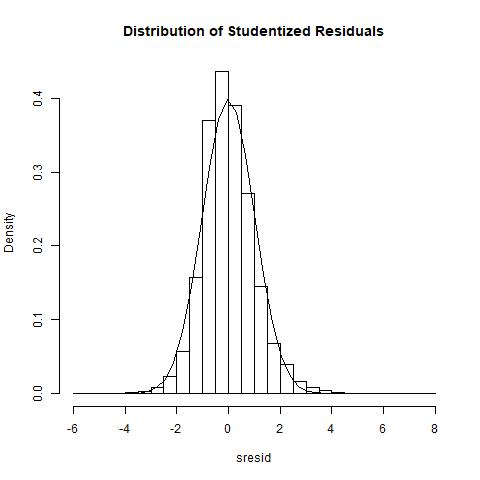
\includegraphics[width= .6\linewidth]{images/student_resid_plot.jpeg}
    \caption{Studentized Residuals}
    \label{fig: student_resid}
\end{figure}

\begin{figure}[H]
    \centering
    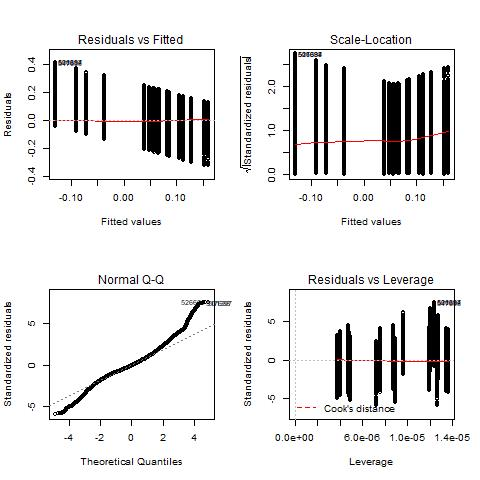
\includegraphics[width= .8\linewidth]{images/plot_matrix.jpeg}
    \caption{Plots of Tests of the Model}
    \label{fig: student_resid}
\end{figure}




\begin{figure}[H]
    \centering
    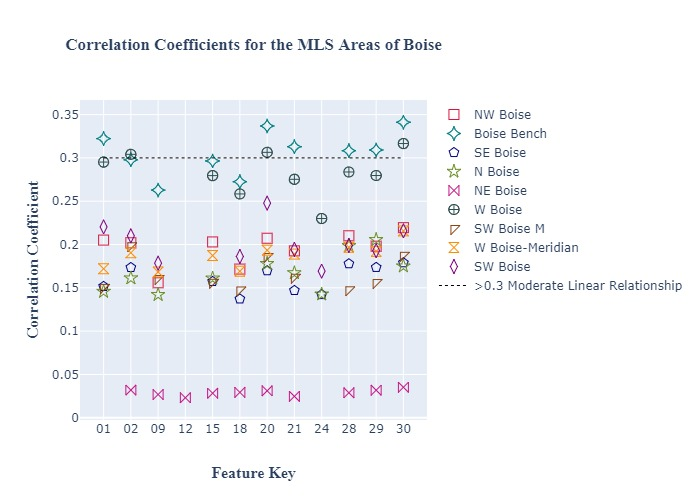
\includegraphics[width= .7\linewidth]{images/Area_fig.jpg}
    \caption{Correlation Coefficients for MLS Areas of Boise}
    \label{fig: area_ccl}
\end{figure}

\begin{figure}[H]
    \centering
    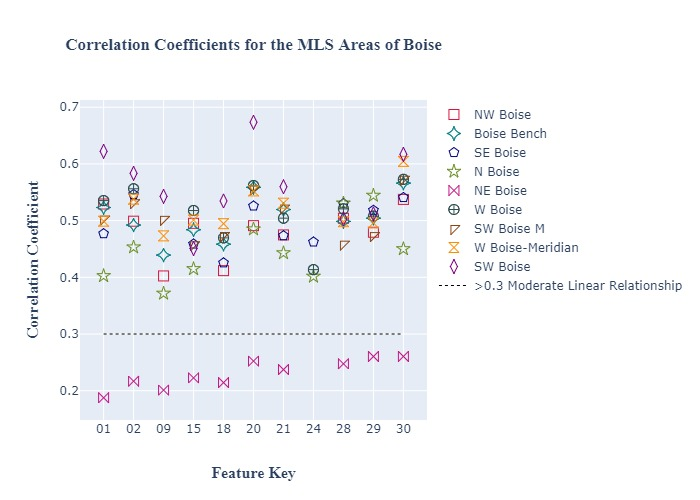
\includegraphics[width= .7\linewidth]{images/Ex_Area_fig.jpg}
    \caption{Correlation Coefficients for MLS Areas of Boise with z-score trim}
    \label{fig: area_ccl-z}
\end{figure}

\begin{figure}[H]
     \centering
     \begin{subfigure}[b]{0.45\textwidth}
         \centering
         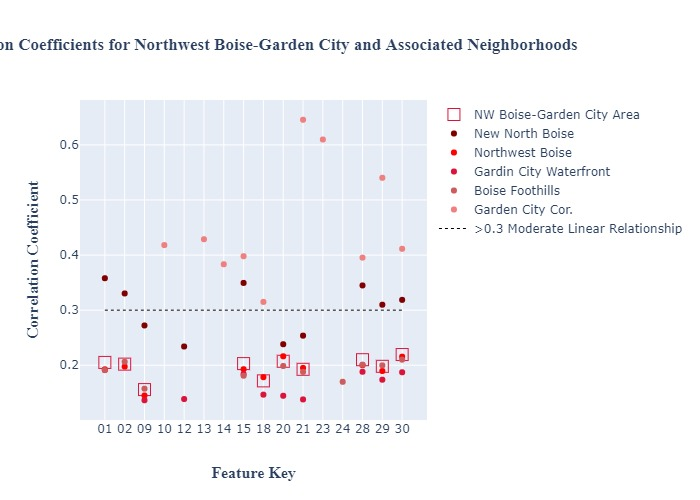
\includegraphics[width=\textwidth]{images/NW_fig.jpg}
         \caption{Northwest Boise Area \& Associated Neighborhoods}
         \label{fig: nw_cc}
     \end{subfigure}
     \begin{subfigure}[b]{0.45\textwidth}
         \centering
         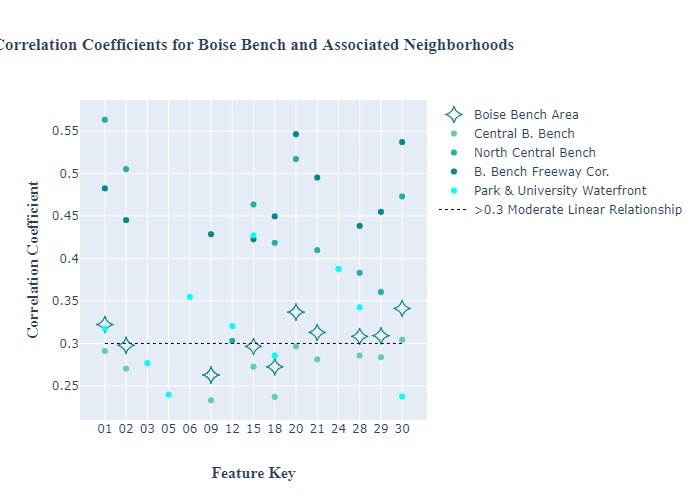
\includegraphics[width=\textwidth]{images/BB_fig.jpg}
         \caption{Boise Bench Area \& Associated Neighborhoods}
         \label{fig: bb_cc}
     \end{subfigure}
          \begin{subfigure}[b]{0.45\textwidth}
         \centering
         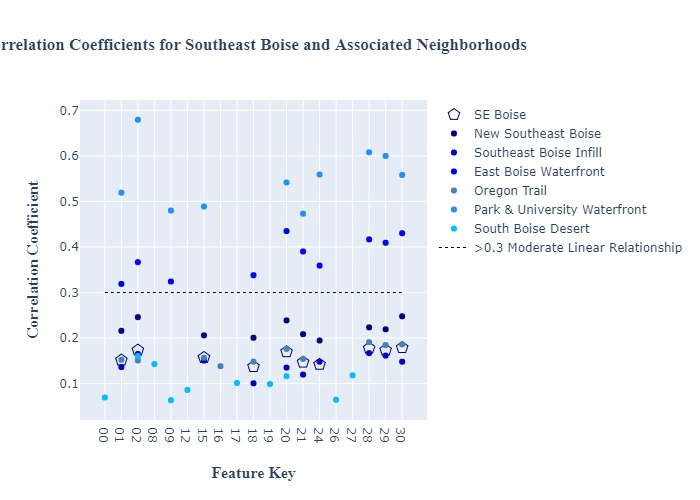
\includegraphics[width=\textwidth]{images/SEB_fig.jpg}
         \caption{Southeast Boise Area \& Associated Neighborhoods}
         \label{fig: se_cc}
     \end{subfigure}
          \begin{subfigure}[b]{0.45\textwidth}
         \centering
         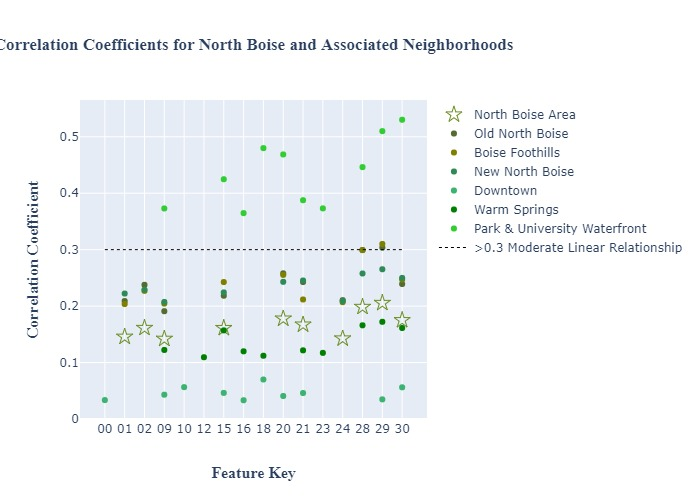
\includegraphics[width=\textwidth]{images/NB_fig.jpg}
         \caption{North Boise Area \& Associated Neighborhoods}
         \label{fig: nb_cc}
     \end{subfigure}
               \begin{subfigure}[b]{0.45\textwidth}
         \centering
         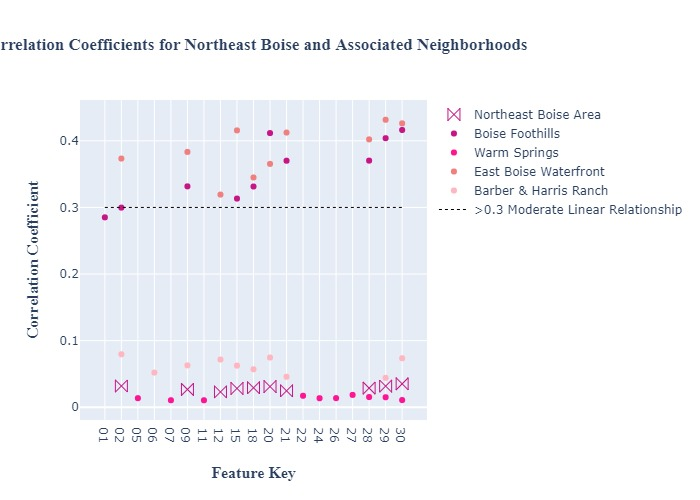
\includegraphics[width=\textwidth]{images/NE_fig.jpg}
         \caption{Northeast Boise Area \& Associated Neighborhoods}
         \label{fig: ne_ccg}
     \end{subfigure}
               \begin{subfigure}[b]{0.45\textwidth}
         \centering
         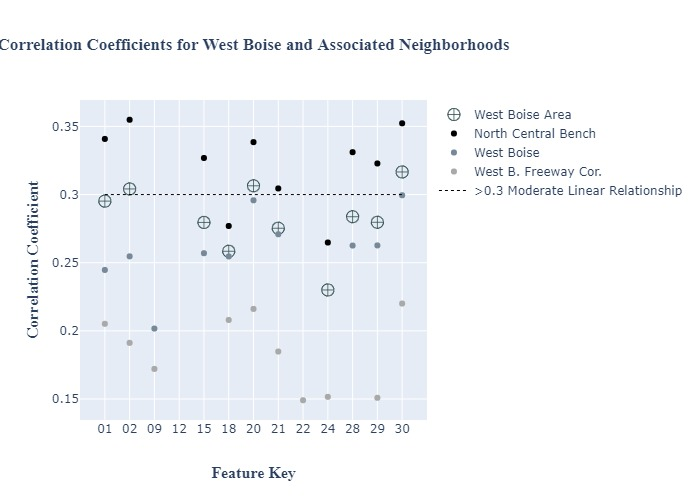
\includegraphics[width=\textwidth]{images/WB_fig.jpg}
         \caption{West Boise Area \& Associated Neighborhoods}
         \label{fig: wb_ccg}
     \end{subfigure}
               \begin{subfigure}[b]{0.45\textwidth}
         \centering
         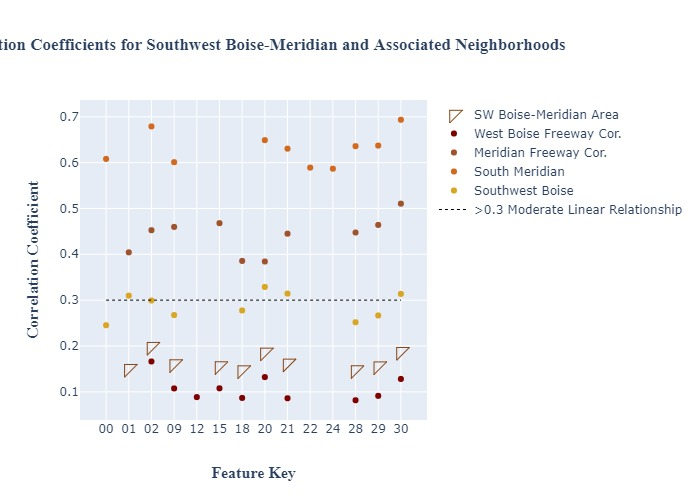
\includegraphics[width=\textwidth]{images/SWBM_fig.jpg}
         \caption{Southwest Boise-Meridian Area \& Associated Neighborhoods}
         \label{fig: swbm_ccg}
     \end{subfigure}
               \begin{subfigure}[b]{0.45\textwidth}
         \centering
         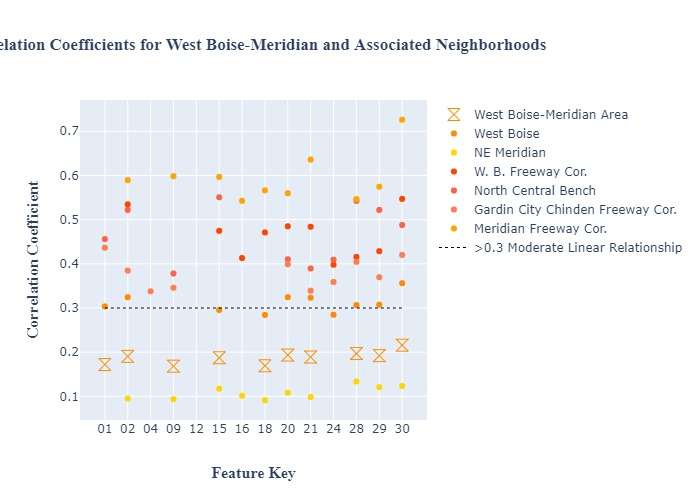
\includegraphics[width=\textwidth]{images/WBM_fig.jpg}
         \caption{West Boise-Meridian Area \& Associated Neighborhoods}
         \label{fig: wbm_ccg}
     \end{subfigure}
               \begin{subfigure}[b]{0.45\textwidth}
         \centering
         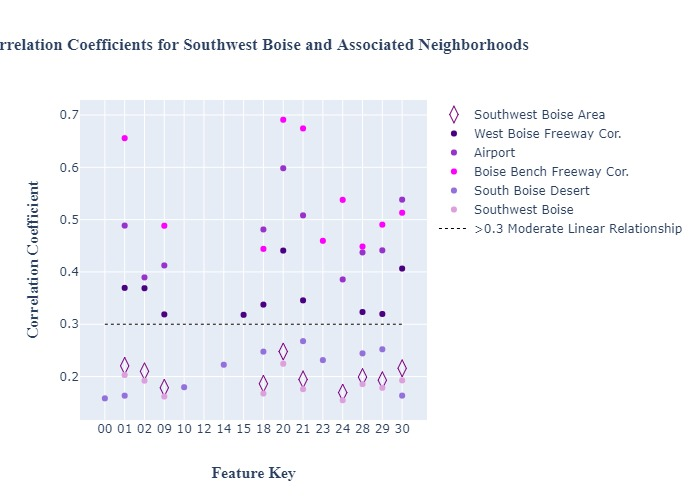
\includegraphics[width=\textwidth]{images/SW_fig.jpg}
         \caption{Southwest Boise Area \& Associated Neighborhoods}
         \label{fig: sw_ccg}
     \end{subfigure}
        \caption{Correlation Coefficients for the Boise Areas and Associated Neighborhoods against chosen features}
        \label{fig: all_ccg}
\end{figure}


\section{Comments and Conclusions}
Tech jobs didn't have the highest VIFF(?).
Further research could dig further into the details of each job category and how the salary increases of that category played into the changes in housing prices.

\appendix
\section{Appendix: Technical Details}



\section{Appendix: Code}

{\footnotesize
\begin{verbatim}
> ### Required packages
> library(car)                                               # required to use scatterplot()
> library(HH)                                                # required to use ci.plot()
>
> ### Read the dataset
> data.skin <- read.table(file=paste(WD.inp,"skincancer.txt",sep=""),header=TRUE)
> data.skin
\end{verbatim}
}

%------------------------------------------------------------------------------%
% References
%------------------------------------------------------------------------------%
\begin{thebibliography}{3}

\bibitem[\protect\astroncite{ACAO}{2019}]{ACAO:2019}
Ada County Assessor's Office (July 8, 2019)
\newblock \textit{Residential House Details for homes in Boise Idaho, from 2000-July 8, 2019}.
% Compiled by Alan Smith Strategic Development Analyst
%\newblock 


\bibitem[\protect\astroncite{KWR}{2019}]{KWR:2019}
Keller Williams Reality Boise (August 6, 2019)
\newblock \textit{Boise Neighborhood Guide}.
\newblock \url{https://www.weknowboise.com/boise-neighborhoods.php}


\bibitem[\protect\astroncite{BLS}{2019}]{BLS:2019}
United States Bureau of Labor Statistics (August 3, 2019)
\newblock \textit{Occupational Employment Statistics}.
% Last Modified Date: March 29, 2019
\newblock \url{https://www.bls.gov/oes/tables.htm}

\bibitem[\protect\astroncite{USC}{2019}]{USCB:2019}
United States Census Bureau, Population Division (August 4, 2019)
\newblock \textit{Annual Estimates of Housing Units for the United States, Regions, Divisions, States, and Counties: April 1, 2010 to July 1, 2018 Release Date: May 2019}.
% https://factfinder.census.gov/faces/tableservices/jsf/pages/productview.xhtml?pid=PEP_2018_PEPANNHU&prodType=table
%\newblock \url{https://www.bls.gov/oes/tables.htm}
%https://www.census.gov/data/tables/time-series/demo/popest/intercensal-2000-2010-housing-units.html


%https://www.ktvb.com/article/news/wall-street-journal-notes-red-hot-boise-housing-market/277-bf82d25c-334b-432c-ace6-7480dd3f5c86



\bibitem[\protect\astroncite{Chen and Wu}{2008}]{Chen:Wu:2008}
Chen, J. and Wu, H. (2008)
\newblock Efficient local estimation for time-varying coefficients in
deterministic dynamic models with applications to {HIV}-1 dynamics.
\newblock \textit{Journal of the American Statistical Association}, 103, 369--384.

\bibitem[\protect\astroncite{Shumway and Stoffer}{2011}]{Shumway:Stoffer:2011}
Shumway, R. H. and Stoffer, D. S. (2011)
\newblock \textit{Time Series analysis and Its Applications With R Examples}, 3rd edn.
\newblock New York: Springer.
\end{thebibliography}
%-----------------------------------------------------------------------------%
\end{document}
%-----------------------------------------------------------------------------%
    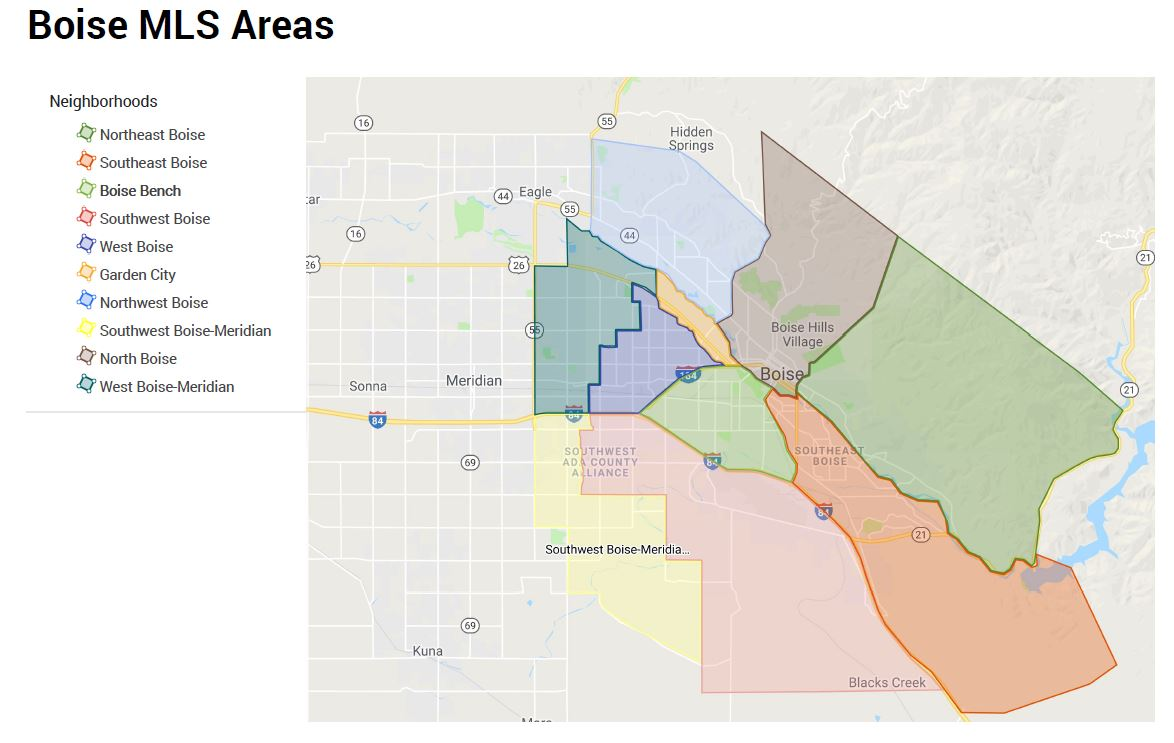
\includegraphics[width= .7\linewidth]{images/MLS_Areas.JPG}

